\documentclass[uplatex,dvipdfmx]{jsarticle}

\usepackage[uplatex,deluxe]{otf} 
% \usepackage[noalphabet]{pxchfon} % Remove to avoid font conflicts
% \usepackage{stix2} % Remove to avoid font conflicts
\usepackage[fleqn,tbtags]{mathtools} 
\usepackage{amsmath}
\usepackage{url}
\usepackage{float} 

\setcounter{tocdepth}{3}
\usepackage{moreverb}
\usepackage{lscape}
\usepackage{ascmac}
\usepackage{xurl}
\usepackage{graphicx} % 画像挿入用

\begin{document}
\title{塩澤匠生の生態に関する調査報告書}
\author{佐土駿}
\date{\today}
\maketitle

\tableofcontents
\newpage    
\section{はじめに}
本報告書は、塩澤匠生の生態に関する調査結果をまとめたものである.調査は2025年4月から2025年10月までの期間にわたり,観察とインタビューを通じて行われた.
ここまででわかった問題点として,カラオケと食に脳が汚染され,死亡リスクが高まっていることが挙げられる.
目的としては,塩澤匠生の行動パターン,趣味,社会的関係を明らかにし,その特徴を理解することである.
これにより,彼の健康状態を改善し,生活の質を向上させるための提案を行うことを目指す.

\section{調査方法}
調査は主に以下の方法で行われた.
\begin{itemize}
    \item 観察: 日常生活の様子を観察し,行動パターンを記録した.
    \item インタビュー: 塩澤匠生本人および彼の友人にインタビューを実施し,趣味や社会的関係についての情報を収集した.
    \item 文献調査: 彼の過去の活動や発言に関する資料を収集し,分析した.
\end{itemize}

\section{調査結果}
\subsection{行動パターン}
\begin{figure}[H]
    \centering
    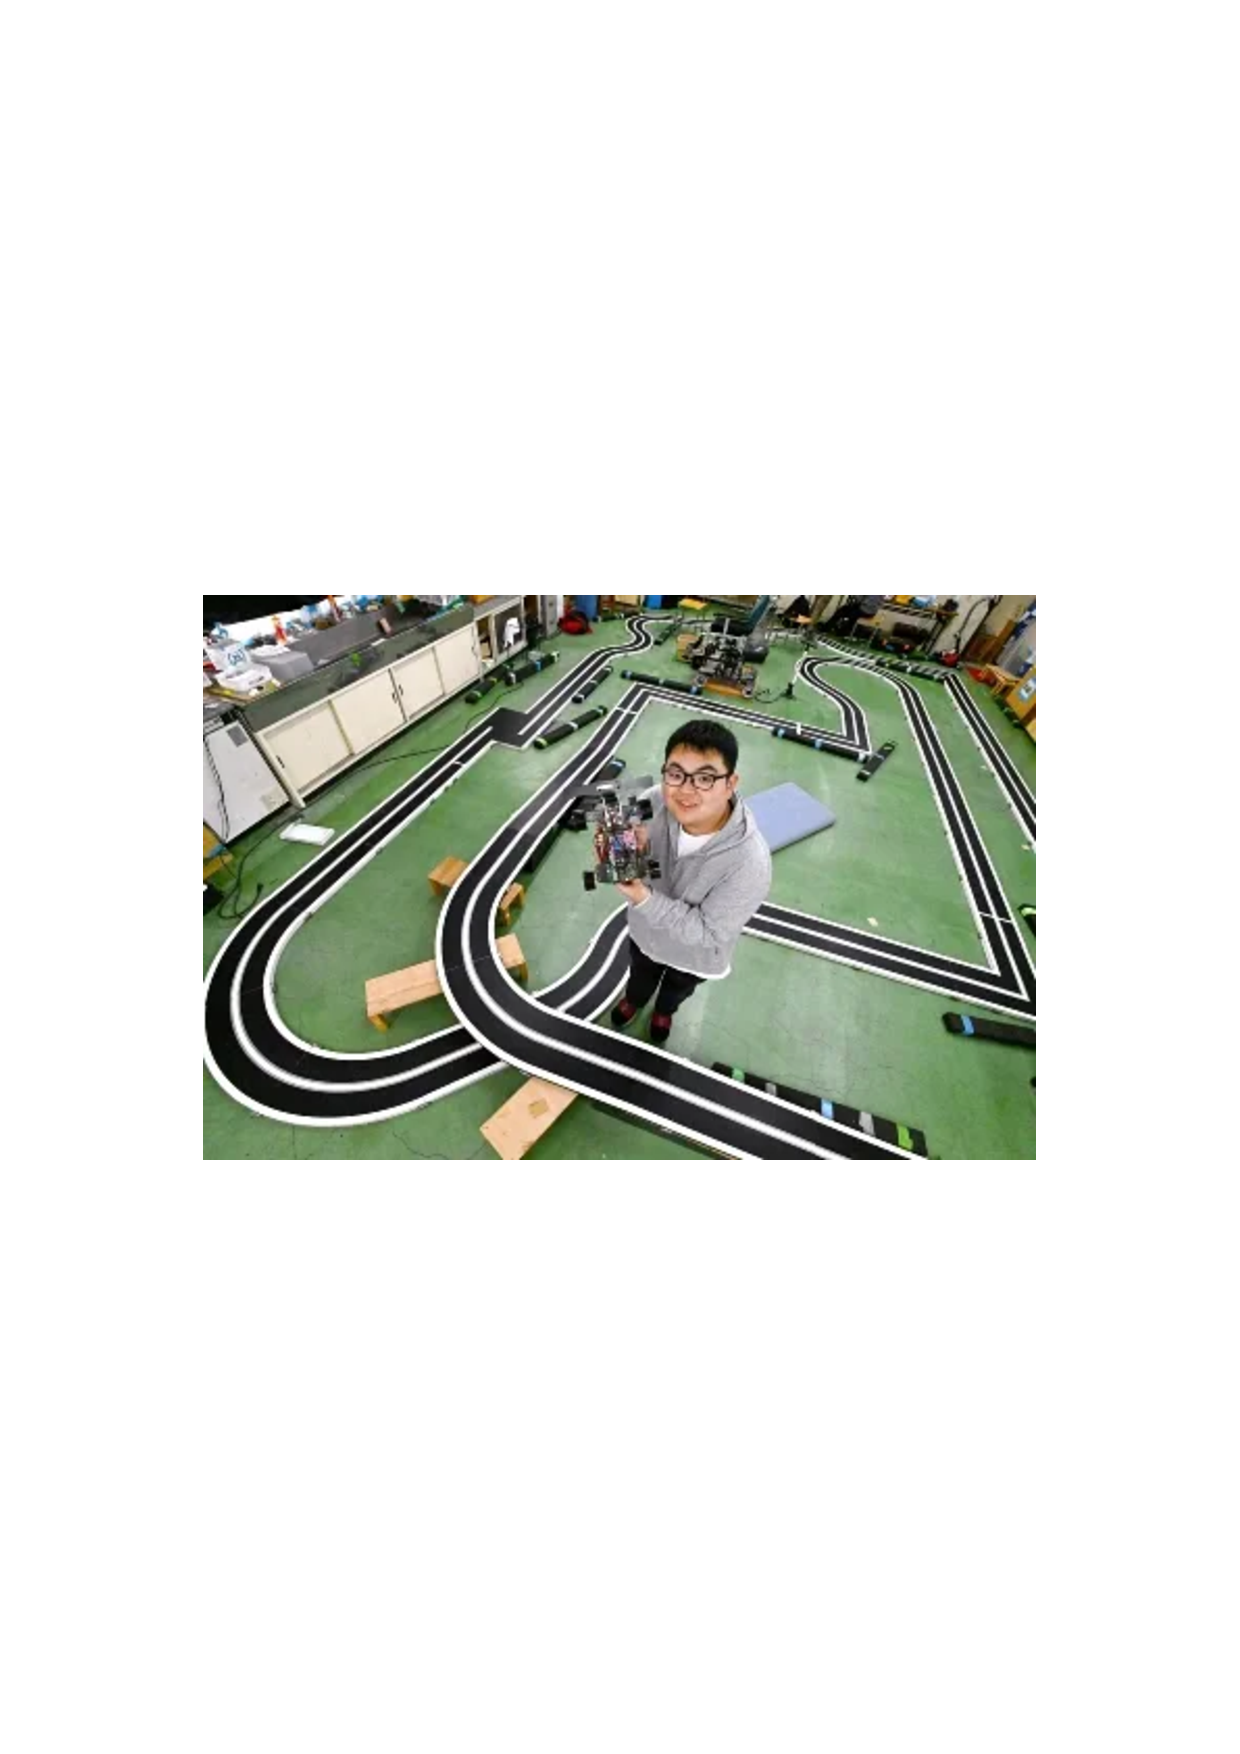
\includegraphics[width=0.5\textwidth]{shiotaku_1.pdf}
    \caption{塩澤匠生の写真}
    \label{fig:shiotaku}
\end{figure}
塩澤匠生は,日常的にカラオケに頻繁に通い,最近では週に1回以上のペースで訪れていることが確認された.また,食事に関しても,高カロリーなファストフードを好む傾向が強く,栄養バランスの取れた食事を摂ることが少ない.これらの行動は,彼の健康状態に悪影響を及ぼしている可能性がある.
また,精神的なストレスを感じている様子も観察され,これが彼の行動に影響を与えている可能性がある.
実際に,習志野市から船橋市までの間を無意識に徒歩移動したという報告もある.
\subsection{趣味}
塩澤匠生の主な趣味はカラオケであり,特にAimerを好んで歌う傾向がある.
2025年前期の単位をすべて取得済みなこともあり,後期の補習がないため,カラオケに費やす時間が増加している.
しかし,アイデアソンという科目は学科での不合格率が9割ほどであり,
金曜日はカラオケに同行する人が存在しない\cite{ref:ideathon}.
また,工業高校出身であることから,技術的な趣味も持っているが,自己肯定感が低く
たまに落ち込む節もある\cite{ref:kougyou}.

\begin{thebibliography}{9}
\bibitem{ref:ideathon} manaba, 「アイデアソン」, \url{https://cit.manaba.jp/ct/course_1474431}
\bibitem{ref:kougyou} SBC信越放送, 「「電気系部活の甲子園」で目指すは日本一 高校生活の集大成となる最速のマイコンカー作りへ 岡工電気部の3人が大会前に熱い思いで続ける微調整」, \url{https://newsdig.tbs.co.jp/articles/sbc/1616586?display=1}
\end{thebibliography}
\end{document}